\chapter{Angle calculation}
\label{chap:angle}

\section{Calculation of the orientation angles}
\label{sec:CalcAngle}
The Kalman filter and the complementary filter need both angles as input. Those angles are calculated with the acceleration sensor and with the gyroscope. The gyroscope sensor is used as main input and is corrected by the acceleration/magnetic sensor. The reason why both are used is already described in the Sensor fusion chapter.\\
To achieve an angle from the gyroscope, the values from the sensor needs to be integrated. The following formulas show the integration part of the function of the gyroscope which runs on the Raspberry Pi. It is located in the folder 'sig/Orientientation/' in the file Orientation.c in the function 'm\_sigOri\_calcGyroAnglePerStep\_st()'. This function calculates the angle which since the last call is made.
\begin{align}
roll_{angle}&=roll_{rate}*deltaT\\
pitch_{angle}&=pitch_{rate}*deltaT\\
yaw_{angle}&=yaw_{rate}*deltaT
\end{align}
To make this code independent from any timestep, it calculates locally the time difference 'deltaT' between the last call. To make this possible the 'gettimeofday' function is used. Because of that any jitter will not make a problem. Also the gyroscope sensor gets automatically offset corrected when the code is started.\\\\
To get an angle from the acceleration/magnetic sensor the following calculation is needed. It is located in the function 'm\_sigOri\_calcAccMagAngle\_st()' in the same file like mentioned before.\\
First the roll angle is calculated:
\begin{align}
roll_{angle\_rad}&=atan2\left(\frac{acc_{y\_axis}}{acc_{z\_axis}}\right)\\
		roll_{angle\_deg}&=-roll_{angle\_rad}*180/Pi
\end{align}

Then the pitch is calculated:
\begin{align}
pitch_{angle\_rad}&=atan\left(-\frac{acc_{x\_axis}}{acc_{y\_axis}*sin(roll_{angle\_rad})+acc_{z\_axis}*cos(roll_{angle\_rad})}\right)\\
pitch_{angle\_deg}&=-pitch_{angle\_rad}*180/Pi
\end{align}

Last step is the calculation of the yaw angle. The yaw angle can not be calculated by the acceleration sensor, only the magnetic sensor can be used for this. But the magnetic sensor can not directly be used. Additional a magnetic tilt compensation needs to be done. The following formulas show the calculation steps.\\
\begin{align}
divider=mag_{x\_axis}&*cos(pitch_{angle\_rad})+\\
mag_{y\_axis}&*sin(pitch_{angle\_rad})*sin(roll_{angle\_rad})+\\
mag_{z\_axis}&*sin(pitch_{angle\_rad})*cos(roll_{angle\_rad})
\end{align}
\begin{align}		
yaw_{angle\_rad}&=atan2\left(\frac{mag_{z\_axis}*sin(roll_{angle\_rad})-mag_{y\_axis}*cos(roll_{angle\_rad})}{divider}\right)\\
yaw_{angle\_deg}&=yaw_{angle\_rad}*180/Pi
\end{align}
With this, the implementation of the fusion filter were done and proved. First the results seem to be correct like can be seen in figure \ref{fig:initial_angle}.

\begin{figure}[H]
	\centering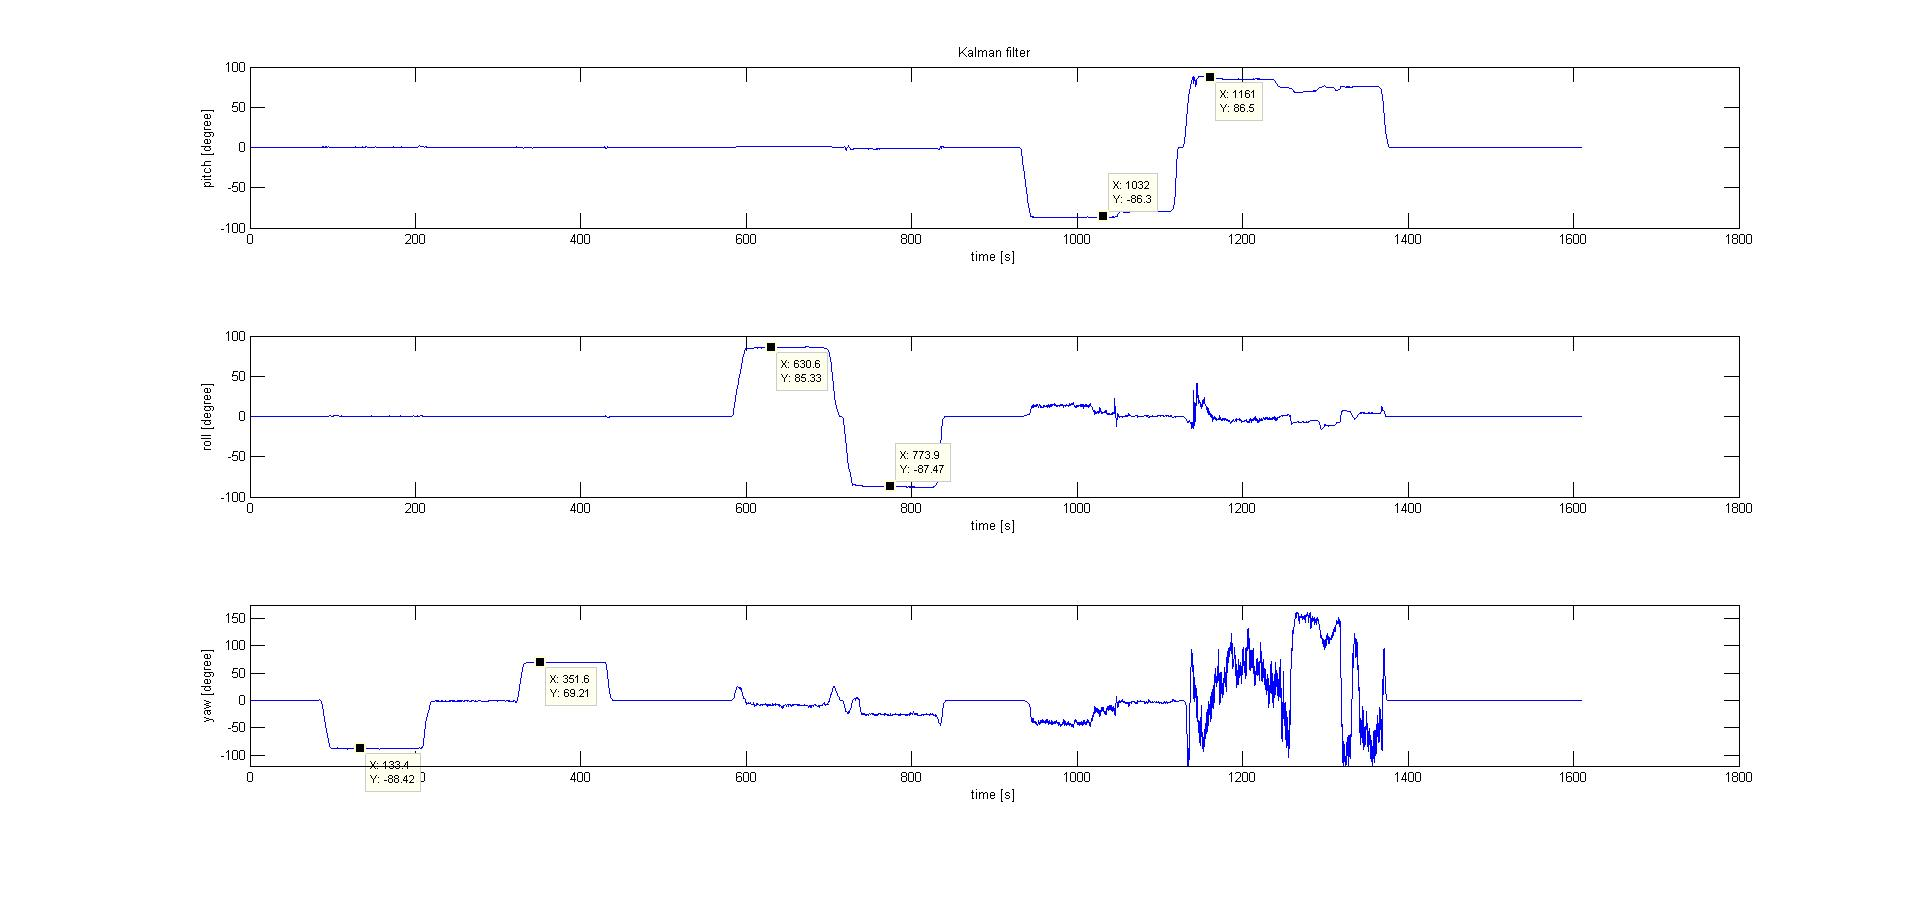
\includegraphics[width=1.0\textwidth]{fig/initial_Kalman}
	\caption{First result Kalman filter}
	\label{fig:initial_angle}
\end{figure}
\section{Magnetic sensor test}
\label{sec:MagSensTest}
As can be seen there is a problem with the yaw angle when a pitch angle is applied. This is no solution which can be used in the quadrocopter. So additional tests are made. After some time the problem was detected. Because just the yaw angle makes some problem, the main observation layed on the magnetic sensor. Figure \ref{fig:field_weak} shows the measured magnetic field.
\begin{figure}[H]
	\centering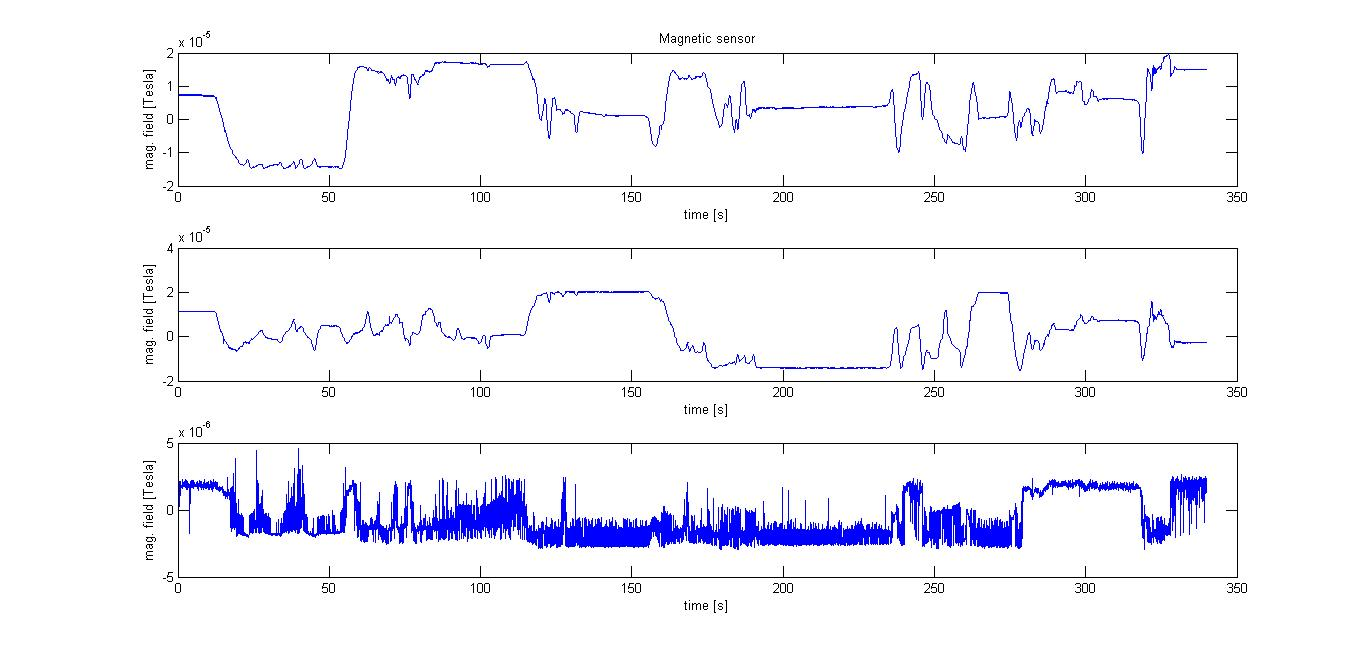
\includegraphics[width=1.0\textwidth]{fig/field_weak}
	\caption{Weak magnetic field strength}
	\label{fig:field_weak}
\end{figure}
The problem can directly be seen. The measured field strength should be nearly the same on all axis. The field strength on the x-axis and y-axis is the same. The z-axis delivers only just one tenth of the normal value. Because of that the noise on the sensor is in the same height like the signal and therefor aquiring not possible. First the position of the mounted IMU is disputed.
After changing the following sensor values of the magnetic sensor can be achieved.
\begin{figure}[H]
	\centering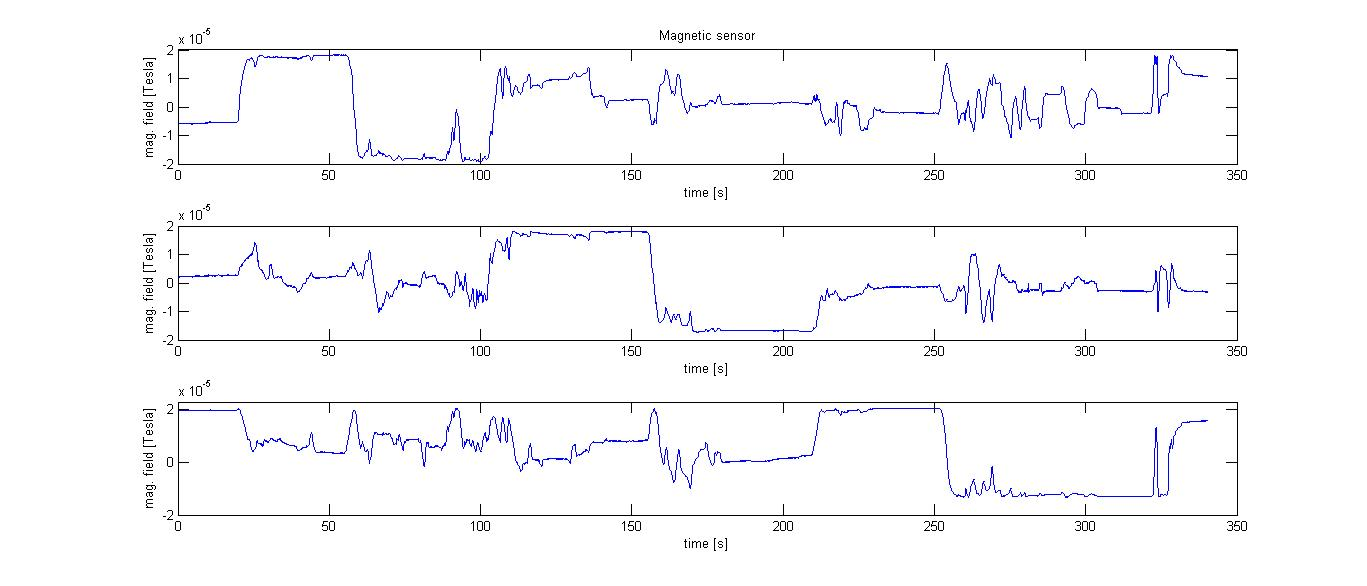
\includegraphics[width=1.0\textwidth]{fig/field_strong}
	\caption{Strong magnetic field strength}
	\label{fig:field_strong}
\end{figure}
By comparing the measurement of the initial positioning of the IMU with the new one, the strength on the z-axis is significantly higher. Also the strength on the three axis are nearly the same. So for further usage the new position is used. 

\section{Improvement magnetic sensor}
\label{sec:ImpMagSens}
The figures \ref{fig:pos_neu1} and \ref{fig:pos_neu2} shows the comparison of the mounting.
\begin{figure}[H]
	\centering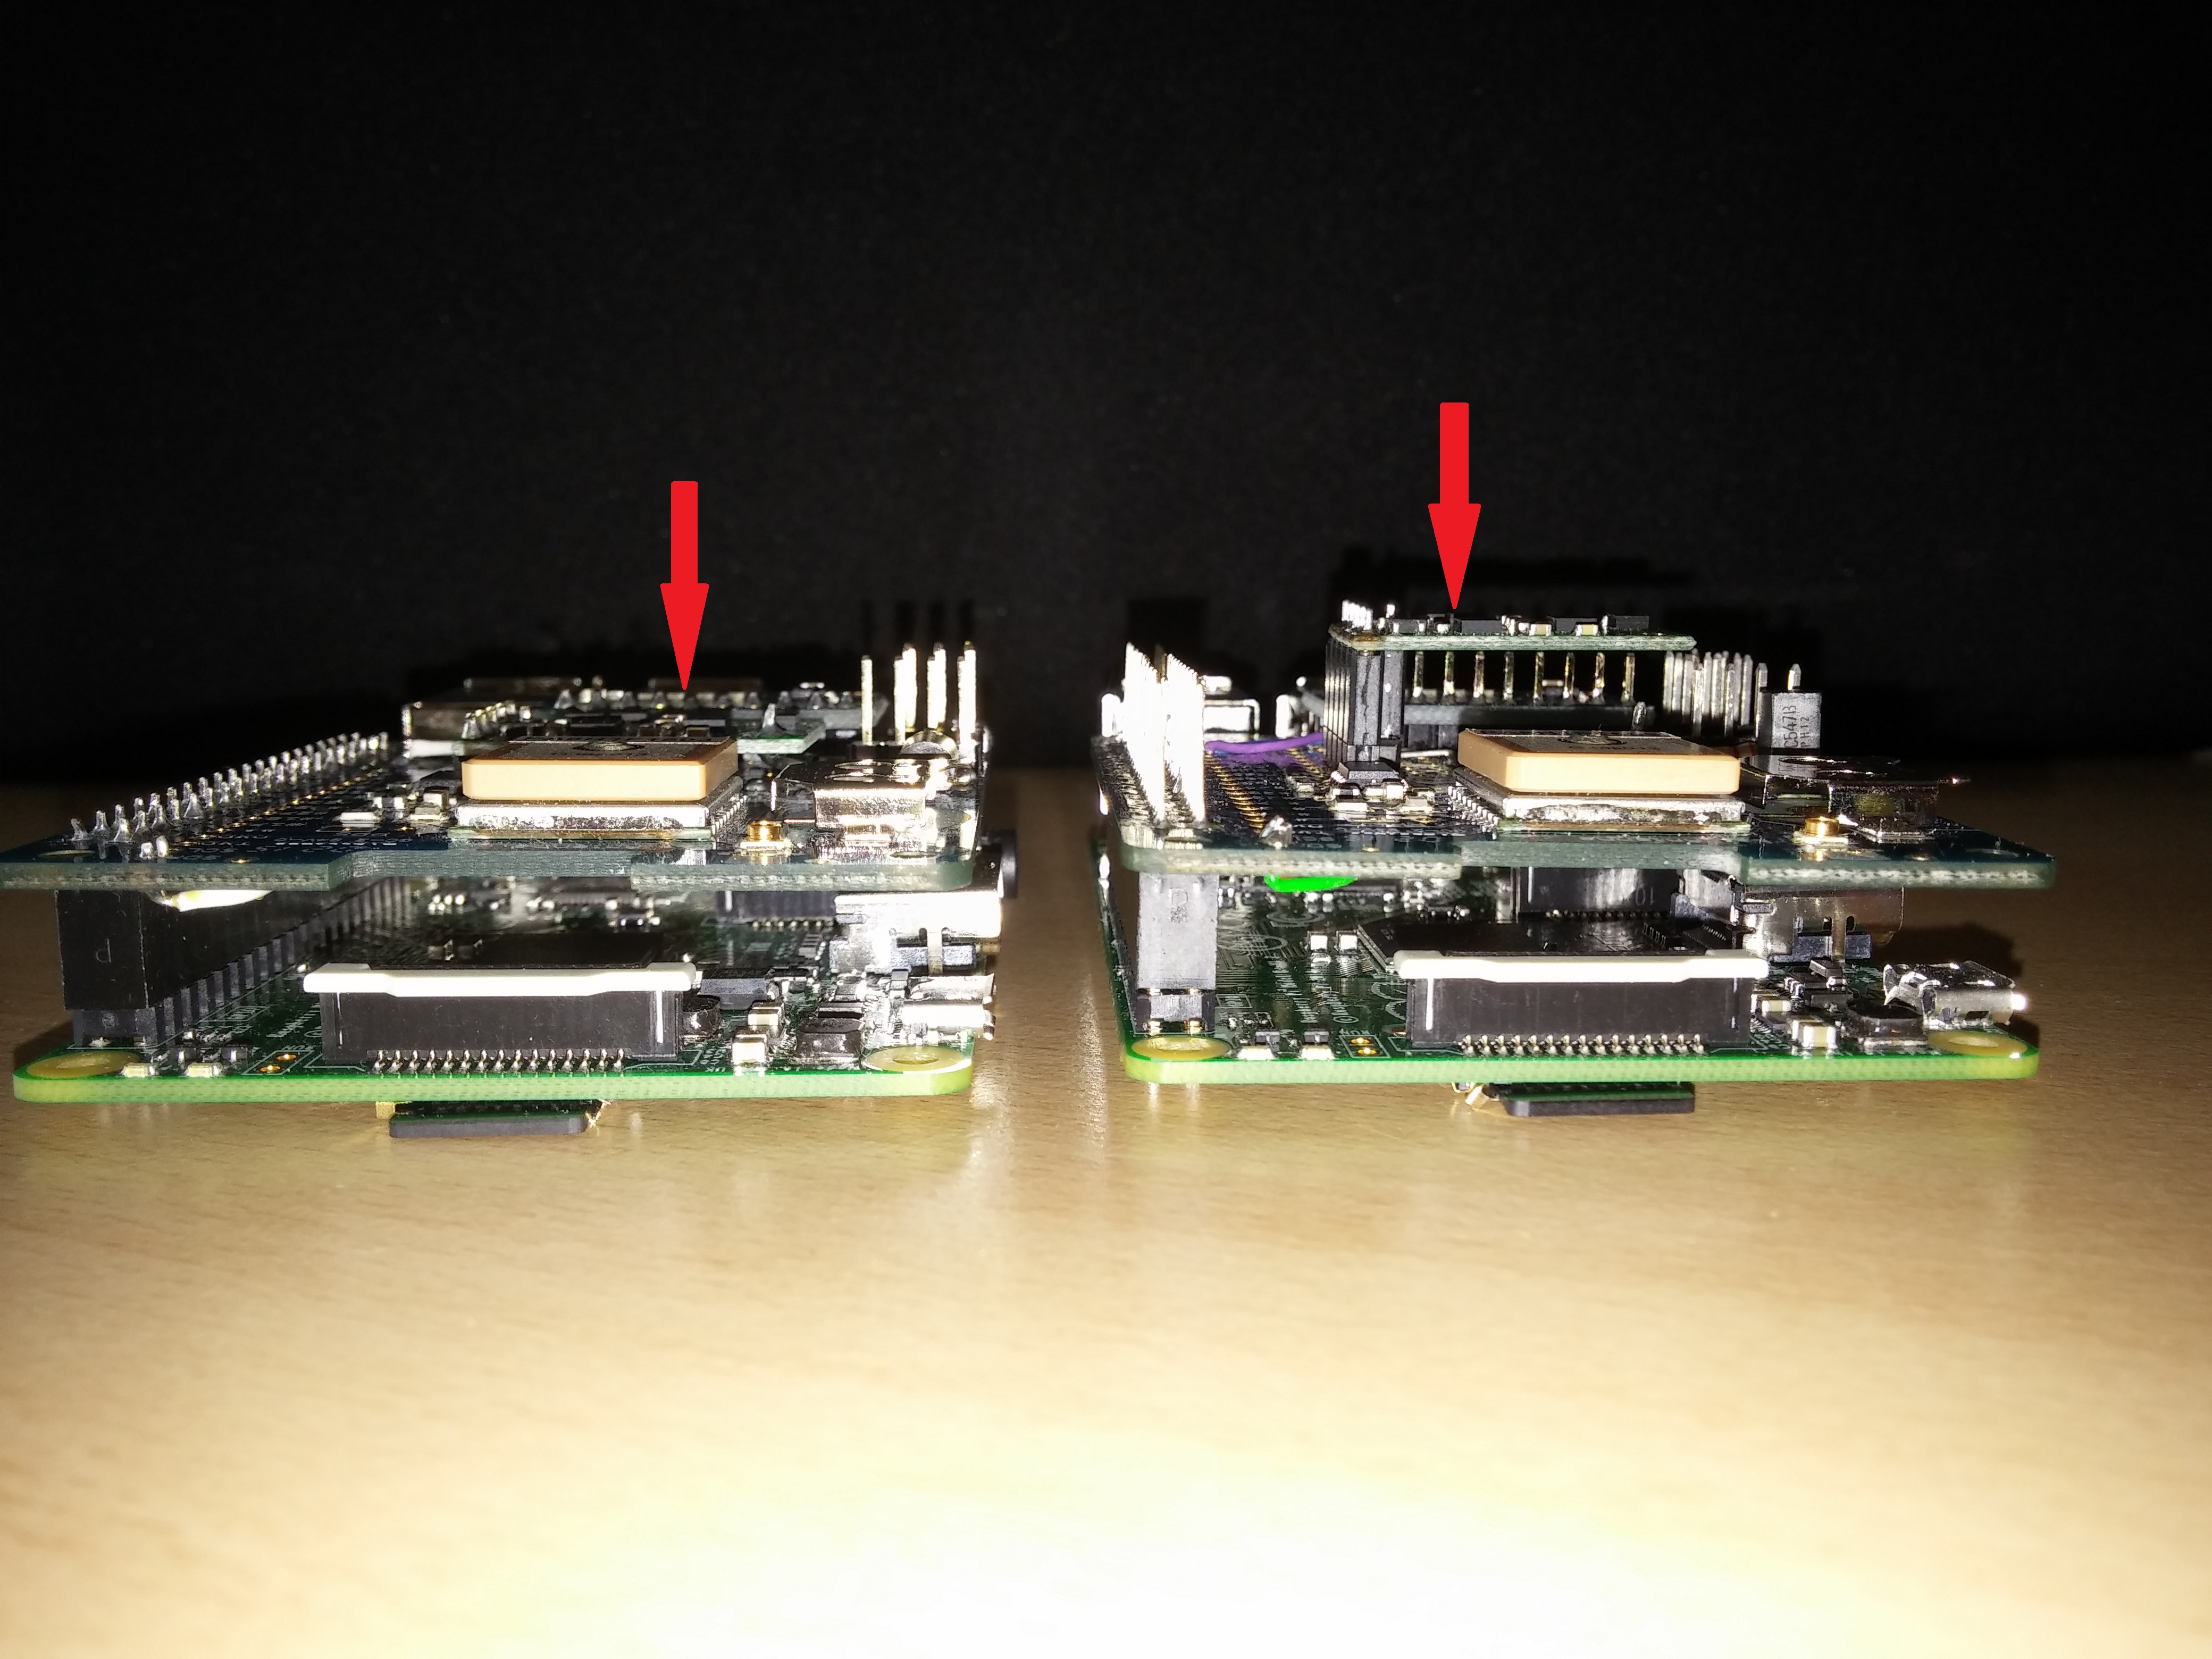
\includegraphics[width=0.6\textwidth]{fig/pos_neu1}
	\caption{New positioning of IMU 1}
	\label{fig:pos_neu1}
\end{figure}
\begin{figure}[H]
	\centering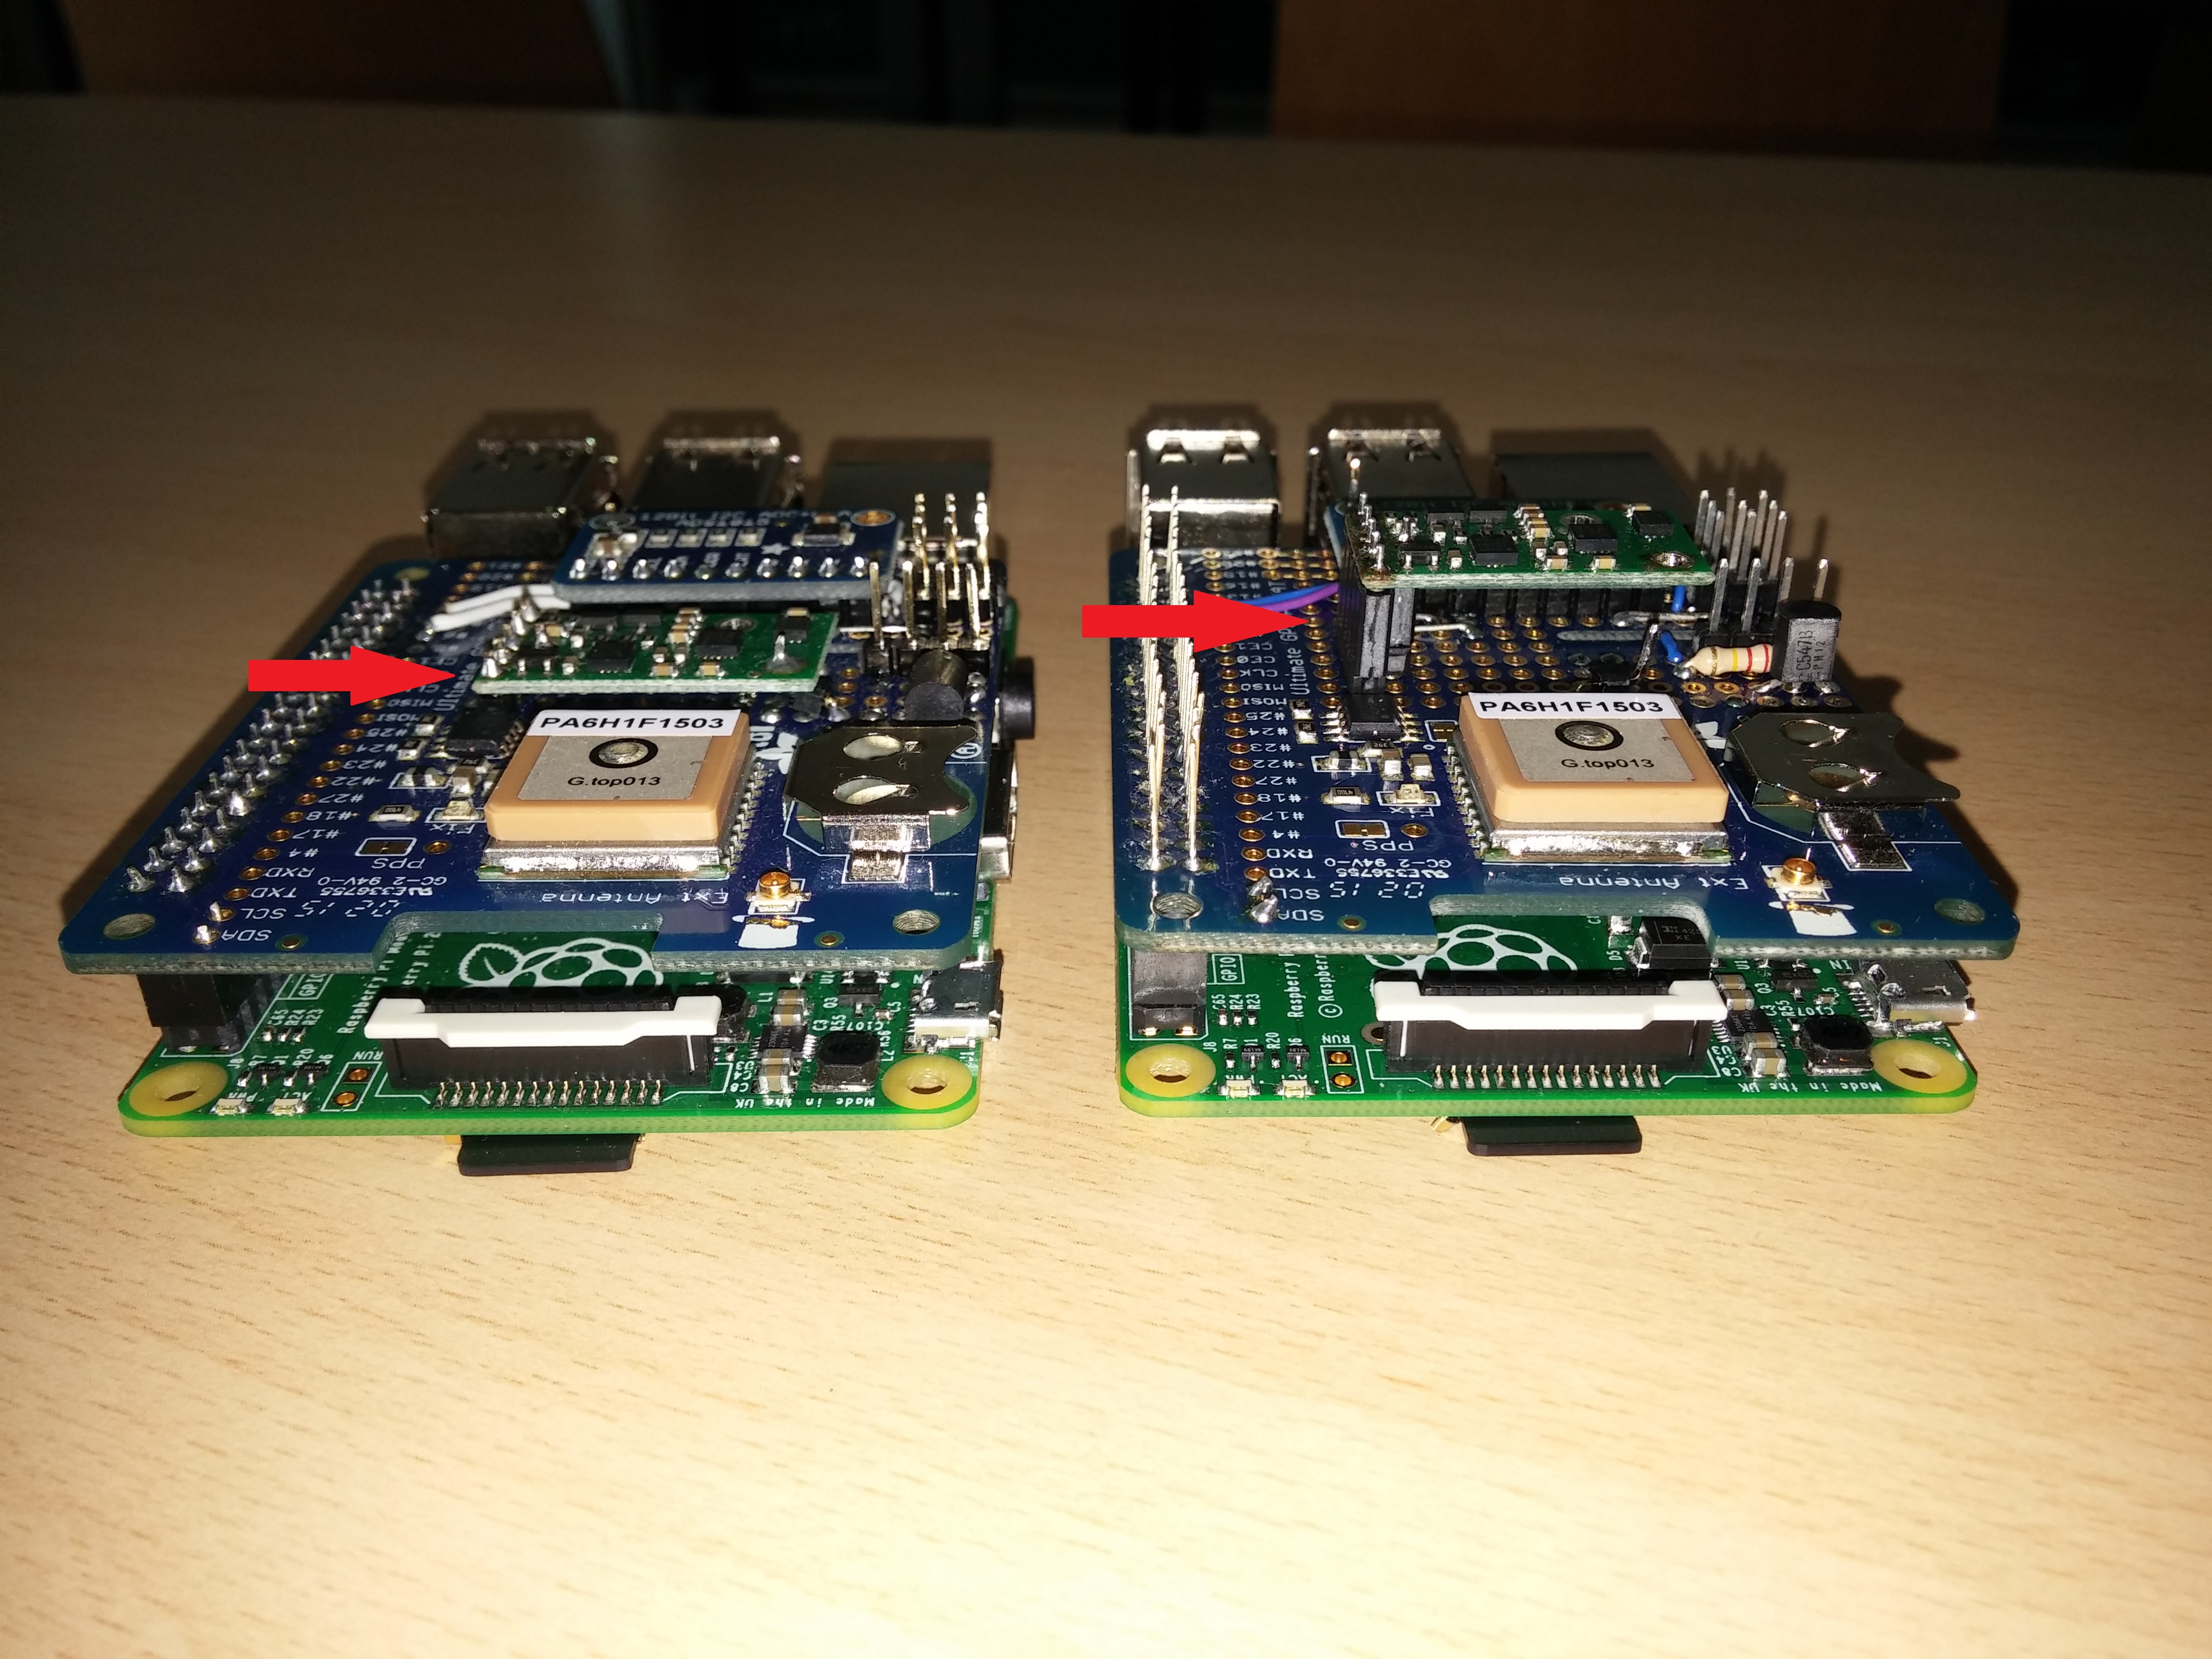
\includegraphics[width=0.6\textwidth]{fig/pos_neu2}
	\caption{New positioning of IMU 2}
	\label{fig:pos_neu2}
\end{figure}
The left PCB shows the old position and the right the new position. As can be seen just the height of the mounted IMU has to be changed. Due to the tests a distance of approximately 1cm seems to be enough. So the wiring can be kept as it is.\\
Additionally to reduce the really high influences of near metallic parts, a hard magnetic offset compensation needs to be done. Also a scaling is done. The following calculations which run in the function 'm\_sigOri\_calcAccMagAngle\_st()' are done within every step.
\begin{align}
mag_{x\_axis}=(mag_{x\_axis}-logged_{min\_x})/(logged_{max\_x}-logged_{min\_x})*2-1\\
mag_{y\_axis}=(mag_{y\_axis}-logged_{min\_y})/(logged_{min\_y}-logged_{min\_y})*2-1\\
mag_{z\_axis}=(mag_{z\_axis}-logged_{min\_z})/(logged_{min\_z}-logged_{min\_z})*2-1
\end{align}
To achieve the full range of the all three sensors the scope of Matlab can be used. The m-file which is mentioned before creates directly the header-file for the code. The improved results due to the changes which are made here can be seen in the second output of the Kalman filter and complementary filter in chapter \ref{chap:ComplementaryFilter} and \ref{chap:KalmanFilter}.